%% Standalone lecture -- build with:  pdflatex -shell-escape mappings
%% Shared preamble for standalone lecture files.
%%
%% Every lecture begins with %% Shared preamble for standalone lecture files.
%%
%% Every lecture begins with %% Shared preamble for standalone lecture files.
%%
%% Every lecture begins with \input{preamble} and is compiled on its own:
%%     pdflatex -shell-escape <lecture>
%% There is no master lectures.tex any more -- the list of lectures lives in
%% lectures.yaml and is read by the build scripts.

\documentclass[25pt,landscape,footrule]{foils}
\input{macros_gen}
\backgroundsetup{contents={}}

\usepackage{stmaryrd}
\usepackage{ifthen}
\usepackage{pdf14}

% Every figure lives in this course's lectures/figures (consolidated
% 2026-10-08).  Do not add other courses' folders back: when a name exists in
% several folders LaTeX silently takes the first, which mixed old and new
% frames of the same animation.  A missing figure should be a build error.
\graphicspath{{figures/}{../lectures/figures/}}

\date{}

\newcounter{lessoncnt}
\newcommand{\lesson}[1]{\setcounter{page}{1}%
\section{Mathematics of Machine Learning\\%
\vfill
\textcolor{red}{\textit{#1}}
\vfill}}
 and is compiled on its own:
%%     pdflatex -shell-escape <lecture>
%% There is no master lectures.tex any more -- the list of lectures lives in
%% lectures.yaml and is read by the build scripts.

\documentclass[25pt,landscape,footrule]{foils}
%\usepackage[compat2,pdftex]{geometry}
\usepackage[pdftex]{geometry}
\geometry{headsep=-2.5ex,hscale=0.9,bmargin=2.5cm,tmargin=1cm,textwidth=25cm}
\usepackage[pdftex]{xcolor}
\usepackage{pause}
\usepackage{background}
%\usepackage[color=white]{background}
\usepackage{listings}
\usepackage{graphicx}
\usepackage{epsfig}
\usepackage{epstopdf}
\usepackage{bm}
\usepackage{amssymb}
\usepackage{amsfonts}
\usepackage{marvosym}
\usepackage{cite}
\usepackage{pifont}
\usepackage[english]{babel}
\usepackage{amsmath}
\usepackage{amsfonts}
\usepackage{rotating}
\usepackage{listings}
\usepackage{pp4slide}
%\usepackage{hyperref}
\usepackage{pp4link}
\usepackage{fancyvrb}
\usepackage{multido}
\usepackage{calc}
\usepackage{mleftright}
\mleftright % Redefines \left to \mleft and \right to \mright



\thinmuskip=1mu

\newcommand{\bigstrut}{\rule[-0.5\baselineskip]{0pt}{1.2\baselineskip}}
\renewcommand{\ttdefault}{pcr}

\newcommand{\squeeze}{\setlength{\itemsep}{-2pt}}
%\renewcommand{\familydefault}{cmr}
%\renewcommand{\labelitemii}{\textcolor{green}{$\star$}}
\newcommand{\tick}{{\large \ding{51}}}
\newcommand{\cross}{{\large \ding{55}}}
%\DeclareMathAlphabet{\mat}{OT1}{cmss}{bx}{n}
\DeclareMathAlphabet{\mat}{U}{eur}{b}{n}
\newcommand{\figs}{/home/apb/figures}
\newcommand{\stimes}{{\scriptstyle \times}}
\newcommand{\tr}{\textsf{T}}
\newcommand{\e}[1]{{\rm e}^{#1}}
\newcommand{\E}[1]{{\rm e}^{{\displaystyle #1}}}
\newcommand{\av}[2][]{\mathbb{E}_{#1}\left[ #2 \right]}
\newcommand{\Var}[1]{\mathbb{V}\mathrm{ar}\left( #1 \right)}
\newcommand{\pred}[1]{\left\llbracket { \small #1} \right\rrbracket}
\newcommand{\logg}[1]{\log\left( #1 \right)}
\newcommand{\logtwo}[1]{\log_2\left( #1 \right)}
\newcommand{\bra}[1]{\left( #1 \right)}
\newcommand{\prob}[1]{\mathbb{P}\left( #1 \right)}
\newcommand{\Prob}[1]{\mathbb{P}\left( #1 \right)}
\newcommand{\Step}{\mathop{\mat{\Theta}}}
\newcommand\diag{\mathop{\mathrm{diag}}}
\newcommand{\grad}{\bm{\nabla}}
\newcommand{\gradx}{\bm{\nabla}_{\!\!\scriptscriptstyle \bm{x}}}
\newcommand{\gradw}{\bm{\nabla}_{\!\!\scriptscriptstyle \bm{w}}}
\newcommand{\dd}{\mathrm{d}}
\newcommand{\ii}{\mathrm{i}}
\newcommand{\data}{\mathcal{D}}
\newcommand{\class}{\mathcal{C}}
\newcommand{\hypo}{\mathcal{H}}
\newcommand{\indep}{\perp \!\!\!\! \perp}
\newcommand{\pd}[3][\,]{\frac{\partial^{#1}{#2}}{\partial\,{#3}}}
\newcommand{\normal}[1]{\mathcal{N}\!\left( #1 \right)}
\newcommand{\Dist}[2][Binom]{\mathrm{#1}\left( \strut {#2} \right)}
\newcommand{\brackets}[1]{\!\left( #1 \right)}
\newcommand{\KL}[2]{\mathop{\mathrm{KL}}\left(#1 \big\| #2\right)}
\newcommand{\argmax}{\mathop{\mathrm{argmax}}}
\newcommand{\argmin}{\mathop{\mathrm{argmin}}}
\newcommand{\margin}{\Delta}
\lstnewenvironment{matlab}[1][frame=TB]{\lstset{#1}}{}       
%\renewcommand{\emph}[1]{\textcolor{red}{\textbf{#1}}}
\newcommand{\myskip}[1]{}
\newcommand\mycom[2]{\genfrac{}{}{0pt}{}{#1}{#2}}
\newcommand{\jl}{\lstinline[basicstyle=\ttfamily\color{DarkGreen},%
 keywordstyle=\bfseries\ttfamily\color{DarkGreen}]}
\definecolor{EmphColor}{rgb}{0.0,0.0,1.0}
\renewcommand{\emph}[1]{{\color{EmphColor}\textbf{#1}}}
\newcommand{\len}[1]{\| #1 \|}
\newcommand{\inner}[2]{\left\langle {#1}, {#2}\right\rangle}
\newenvironment{psmallmatrix}{\left(\begin{smallmatrix}}{\end{smallmatrix}\right)}
  

\definecolor{DarkGreen}{rgb}{0,0.5,0}
\definecolor{DarkRed}{rgb}{0,0,0.5}
\definecolor{HighLight}{rgb}{1,0,0}     % yellow
\definecolor{TextColor}{rgb}{0.0,0.1,0.1}     % white
\definecolor{TwoColor}{rgb}{0.0,0.5,0.1}      % used for switching colors

\definecolor{HeadLineColor}{rgb}{1.0,0.0,0.0} % cyan
\definecolor{SpecialColor}{rgb}{0.53,0.81,1.0}
\renewcommand{\normalcolor}{\color{HeadLineColor}}

\pausecolors{TwoColor}{TextColor}{HighLight}
\pausecolors{EmphColor}{TextColor}{EmphColor}
\pausecolors{DarkGreen}{DarkGreen}{DarkRed}
\pausecolors{SpecialColor}{white}{HighLight}

\newenvironment{PauseHighLight}{\color{TwoColor}\pausehighlight}{}
\newcommand{\multipdf}[2][width=\linewidth]{\multiinclude[pause=\pauselevel{:+0}\pause,format=pdf,graphics={#1}]{#2}}

\lstdefinelanguage{pseudo}
 {keywords={all,and,begin,break,continue,do,else,elseif,%
     end,endif,endfor,endwhile,%
     exit,false,for,forall,goto,if,%
     or,return,then,true,to,repeat,until,while},%
  comment=[s]{/*}{*/},%
  morecomment=[l]//,%
  morestring=[d]"%
 }[keywords,comments,strings]


\lstloadlanguages{Java,pseudo,Python}
\lstset{
  basicstyle=\footnotesize\ttfamily\color{DarkGreen},
  keywordstyle=\bfseries\footnotesize\ttfamily\color{DarkGreen},
  commentstyle=\footnotesize\it\rmfamily\color{blue},
  language=Java,
  showstringspaces=false
  }


\lstnewenvironment{pseudo}[1][]{\lstset{language=pseudo,mathescape,literate={:=}{{$\gets$}}2 {!}{{$\neg$}}1 {!=}{{\!\!$\neq$\,\,}}2 {<=}{{\!\!$\leq$\,\,}}2 {>=}{{\!\!$\geq$\,\,}}2,escapechar=\#,#1}}{}
\lstnewenvironment{java}[1][]{\lstset{escapechar=\$,#1}}{}
% Python code: the language setting makes # comments use commentstyle.
% Comments stay monospaced: the default italic roman letter-spaces badly
% on listings' fixed columns.
\lstnewenvironment{python}[1][frame=TB]{\lstset{language=Python,
    commentstyle=\footnotesize\ttfamily\color{blue},#1}}{}

\MyLogo{}
%\Restriction{}
%\rightfooter{\hyperlink{overview}{$\square$}}

\newcommand{\keywords}[1]{\vfill{\noindent\it #1}}

\newcounter{outlineitem}
\setcounter{outlineitem}{0}
\newcommand{\outlineitem}[2]{\item%
  \def\targ{\value{emumi}}%
  \ifnum\value{enumi}=\value{outlineitem}%
  \color{HighLight}\textbf{#1}\toptarget{#2}\color{TextColor}%
   \else\toplink{#2}{#1}\fi
}
\color{TwoColor}


%-- Instead of writing \section we want the file structured by \section.
\newcommand{\section}[2][0]{\foilhead[#1cm]{#2}}

%-- Write each page into a \begin{slide} -- \end{slide} environment.
\newenvironment{slide}{}{\pauselevel{=1}}

\MyLogo{\pauselevel{=1}\Acrobatmenu{GoBack}{%
  \color{TextColor}{Adam Pr\"ugel-Bennett}} \hspace{2cm}
  % Clicking on the name steps one slide back.
  \toplink{firstoutline}{\color{red}Mathematics of Machine
    Learning}%
  \hspace{2cm}
  \texttt{//ecs-vlc.github.io/aice3001/}
  %Clicking on the date jumps to the last page, which should be the
  %table of contents.
  \rightfooter{\Acrobatmenu{LastPage}{\qquad%
  \textsf{\color{TextColor}\tiny\thepage}}}% page number
  % Clicking on the page number steps one slide back.
}
\raggedright
\newcommand{\Outline}{}

\newcommand{\pb}{\pausebuild \color{TwoColor}}
\newcommand{\pauseb}{\pauselevel{build, highlight}\pause}
\newcommand{\hl}[1]{\pauselevel{=1, highlight =1 :1, highlight =#1 :#1}\pause}
\newcommand{\hll}{\pauselevel{=1, highlight =1 :1}\pause}
\newcommand{\pauseh}{\pauselevel{highlight}\pause}
\newcommand{\nhl}[1]{\textcolor{TextColor}{#1}}
\newcommand{\mypl}[1]{\pauselevel{=#1 :#1}\pause}
\input supp-pdf.tex
\DeclareGraphicsRule{*}{mps}{*}{}
\usepackage{mpmulti}
%\leftheader{}
\rightheader{} % no more page numbers on top right


\hypersetup{pdftitle={ECS Lectures},pdfsubject={Machine Learning}
pdfauthor={Adam Prugel-Bennett},pdfkeywords={machine learning},
pdfpagemode={FullScreen},
bookmarksopen=false,
hypertexnames=false,pdfstartview={FitV},colorlinks,linkcolor={blue},
citecolor={green},urlcolor={blue}}



\newcommand\bluepage{
\clearpage
\renewcommand\normalcolor{\color{yellow}}
\pagecolor{blue}
\renewcommand\Black{\color{white}}
\color{white}
\hypersetup{colorlinks=true}
}

\newcommand\whitepage{
\clearpage
\renewcommand\normalcolor{\color{black}}
\pagecolor{white}
\renewcommand\Black{\color{black}}
\color{black}
\hypersetup{colorlinks=true}
}

\whitepage
\setlength{\unitlength}{1mm}

\newenvironment{leftImage}[2][0.3]{%
\begin{minipage}{#1\linewidth}
  \includegraphics[width=\linewidth]{#2}
\end{minipage}\hfill
\begin{minipage}{0.92\linewidth - #1\linewidth}}%
{\end{minipage}}

\newenvironment{rightImage}[2][0.3]{%
\newcommand{\foot}{\begin{minipage}{#1\linewidth}\includegraphics[width=0.98\linewidth]{#2}\end{minipage}}%
\begin{minipage}{0.95\linewidth - #1\linewidth}\raggedright }{\end{minipage}\hfill\foot}


%%% Local Variables: 
%%% mode: latex
%%% TeX-master: t
%%% End: 

\backgroundsetup{contents={}}

\usepackage{stmaryrd}
\usepackage{ifthen}
\usepackage{pdf14}

% Every figure lives in this course's lectures/figures (consolidated
% 2026-10-08).  Do not add other courses' folders back: when a name exists in
% several folders LaTeX silently takes the first, which mixed old and new
% frames of the same animation.  A missing figure should be a build error.
\graphicspath{{figures/}{../lectures/figures/}}

\date{}

\newcounter{lessoncnt}
\newcommand{\lesson}[1]{\setcounter{page}{1}%
\section{Mathematics of Machine Learning\\%
\vfill
\textcolor{red}{\textit{#1}}
\vfill}}
 and is compiled on its own:
%%     pdflatex -shell-escape <lecture>
%% There is no master lectures.tex any more -- the list of lectures lives in
%% lectures.yaml and is read by the build scripts.

\documentclass[25pt,landscape,footrule]{foils}
%\usepackage[compat2,pdftex]{geometry}
\usepackage[pdftex]{geometry}
\geometry{headsep=-2.5ex,hscale=0.9,bmargin=2.5cm,tmargin=1cm,textwidth=25cm}
\usepackage[pdftex]{xcolor}
\usepackage{pause}
\usepackage{background}
%\usepackage[color=white]{background}
\usepackage{listings}
\usepackage{graphicx}
\usepackage{epsfig}
\usepackage{epstopdf}
\usepackage{bm}
\usepackage{amssymb}
\usepackage{amsfonts}
\usepackage{marvosym}
\usepackage{cite}
\usepackage{pifont}
\usepackage[english]{babel}
\usepackage{amsmath}
\usepackage{amsfonts}
\usepackage{rotating}
\usepackage{listings}
\usepackage{pp4slide}
%\usepackage{hyperref}
\usepackage{pp4link}
\usepackage{fancyvrb}
\usepackage{multido}
\usepackage{calc}
\usepackage{mleftright}
\mleftright % Redefines \left to \mleft and \right to \mright



\thinmuskip=1mu

\newcommand{\bigstrut}{\rule[-0.5\baselineskip]{0pt}{1.2\baselineskip}}
\renewcommand{\ttdefault}{pcr}

\newcommand{\squeeze}{\setlength{\itemsep}{-2pt}}
%\renewcommand{\familydefault}{cmr}
%\renewcommand{\labelitemii}{\textcolor{green}{$\star$}}
\newcommand{\tick}{{\large \ding{51}}}
\newcommand{\cross}{{\large \ding{55}}}
%\DeclareMathAlphabet{\mat}{OT1}{cmss}{bx}{n}
\DeclareMathAlphabet{\mat}{U}{eur}{b}{n}
\newcommand{\figs}{/home/apb/figures}
\newcommand{\stimes}{{\scriptstyle \times}}
\newcommand{\tr}{\textsf{T}}
\newcommand{\e}[1]{{\rm e}^{#1}}
\newcommand{\E}[1]{{\rm e}^{{\displaystyle #1}}}
\newcommand{\av}[2][]{\mathbb{E}_{#1}\left[ #2 \right]}
\newcommand{\Var}[1]{\mathbb{V}\mathrm{ar}\left( #1 \right)}
\newcommand{\pred}[1]{\left\llbracket { \small #1} \right\rrbracket}
\newcommand{\logg}[1]{\log\left( #1 \right)}
\newcommand{\logtwo}[1]{\log_2\left( #1 \right)}
\newcommand{\bra}[1]{\left( #1 \right)}
\newcommand{\prob}[1]{\mathbb{P}\left( #1 \right)}
\newcommand{\Prob}[1]{\mathbb{P}\left( #1 \right)}
\newcommand{\Step}{\mathop{\mat{\Theta}}}
\newcommand\diag{\mathop{\mathrm{diag}}}
\newcommand{\grad}{\bm{\nabla}}
\newcommand{\gradx}{\bm{\nabla}_{\!\!\scriptscriptstyle \bm{x}}}
\newcommand{\gradw}{\bm{\nabla}_{\!\!\scriptscriptstyle \bm{w}}}
\newcommand{\dd}{\mathrm{d}}
\newcommand{\ii}{\mathrm{i}}
\newcommand{\data}{\mathcal{D}}
\newcommand{\class}{\mathcal{C}}
\newcommand{\hypo}{\mathcal{H}}
\newcommand{\indep}{\perp \!\!\!\! \perp}
\newcommand{\pd}[3][\,]{\frac{\partial^{#1}{#2}}{\partial\,{#3}}}
\newcommand{\normal}[1]{\mathcal{N}\!\left( #1 \right)}
\newcommand{\Dist}[2][Binom]{\mathrm{#1}\left( \strut {#2} \right)}
\newcommand{\brackets}[1]{\!\left( #1 \right)}
\newcommand{\KL}[2]{\mathop{\mathrm{KL}}\left(#1 \big\| #2\right)}
\newcommand{\argmax}{\mathop{\mathrm{argmax}}}
\newcommand{\argmin}{\mathop{\mathrm{argmin}}}
\newcommand{\margin}{\Delta}
\lstnewenvironment{matlab}[1][frame=TB]{\lstset{#1}}{}       
%\renewcommand{\emph}[1]{\textcolor{red}{\textbf{#1}}}
\newcommand{\myskip}[1]{}
\newcommand\mycom[2]{\genfrac{}{}{0pt}{}{#1}{#2}}
\newcommand{\jl}{\lstinline[basicstyle=\ttfamily\color{DarkGreen},%
 keywordstyle=\bfseries\ttfamily\color{DarkGreen}]}
\definecolor{EmphColor}{rgb}{0.0,0.0,1.0}
\renewcommand{\emph}[1]{{\color{EmphColor}\textbf{#1}}}
\newcommand{\len}[1]{\| #1 \|}
\newcommand{\inner}[2]{\left\langle {#1}, {#2}\right\rangle}
\newenvironment{psmallmatrix}{\left(\begin{smallmatrix}}{\end{smallmatrix}\right)}
  

\definecolor{DarkGreen}{rgb}{0,0.5,0}
\definecolor{DarkRed}{rgb}{0,0,0.5}
\definecolor{HighLight}{rgb}{1,0,0}     % yellow
\definecolor{TextColor}{rgb}{0.0,0.1,0.1}     % white
\definecolor{TwoColor}{rgb}{0.0,0.5,0.1}      % used for switching colors

\definecolor{HeadLineColor}{rgb}{1.0,0.0,0.0} % cyan
\definecolor{SpecialColor}{rgb}{0.53,0.81,1.0}
\renewcommand{\normalcolor}{\color{HeadLineColor}}

\pausecolors{TwoColor}{TextColor}{HighLight}
\pausecolors{EmphColor}{TextColor}{EmphColor}
\pausecolors{DarkGreen}{DarkGreen}{DarkRed}
\pausecolors{SpecialColor}{white}{HighLight}

\newenvironment{PauseHighLight}{\color{TwoColor}\pausehighlight}{}
\newcommand{\multipdf}[2][width=\linewidth]{\multiinclude[pause=\pauselevel{:+0}\pause,format=pdf,graphics={#1}]{#2}}

\lstdefinelanguage{pseudo}
 {keywords={all,and,begin,break,continue,do,else,elseif,%
     end,endif,endfor,endwhile,%
     exit,false,for,forall,goto,if,%
     or,return,then,true,to,repeat,until,while},%
  comment=[s]{/*}{*/},%
  morecomment=[l]//,%
  morestring=[d]"%
 }[keywords,comments,strings]


\lstloadlanguages{Java,pseudo,Python}
\lstset{
  basicstyle=\footnotesize\ttfamily\color{DarkGreen},
  keywordstyle=\bfseries\footnotesize\ttfamily\color{DarkGreen},
  commentstyle=\footnotesize\it\rmfamily\color{blue},
  language=Java,
  showstringspaces=false
  }


\lstnewenvironment{pseudo}[1][]{\lstset{language=pseudo,mathescape,literate={:=}{{$\gets$}}2 {!}{{$\neg$}}1 {!=}{{\!\!$\neq$\,\,}}2 {<=}{{\!\!$\leq$\,\,}}2 {>=}{{\!\!$\geq$\,\,}}2,escapechar=\#,#1}}{}
\lstnewenvironment{java}[1][]{\lstset{escapechar=\$,#1}}{}
% Python code: the language setting makes # comments use commentstyle.
% Comments stay monospaced: the default italic roman letter-spaces badly
% on listings' fixed columns.
\lstnewenvironment{python}[1][frame=TB]{\lstset{language=Python,
    commentstyle=\footnotesize\ttfamily\color{blue},#1}}{}

\MyLogo{}
%\Restriction{}
%\rightfooter{\hyperlink{overview}{$\square$}}

\newcommand{\keywords}[1]{\vfill{\noindent\it #1}}

\newcounter{outlineitem}
\setcounter{outlineitem}{0}
\newcommand{\outlineitem}[2]{\item%
  \def\targ{\value{emumi}}%
  \ifnum\value{enumi}=\value{outlineitem}%
  \color{HighLight}\textbf{#1}\toptarget{#2}\color{TextColor}%
   \else\toplink{#2}{#1}\fi
}
\color{TwoColor}


%-- Instead of writing \section we want the file structured by \section.
\newcommand{\section}[2][0]{\foilhead[#1cm]{#2}}

%-- Write each page into a \begin{slide} -- \end{slide} environment.
\newenvironment{slide}{}{\pauselevel{=1}}

\MyLogo{\pauselevel{=1}\Acrobatmenu{GoBack}{%
  \color{TextColor}{Adam Pr\"ugel-Bennett}} \hspace{2cm}
  % Clicking on the name steps one slide back.
  \toplink{firstoutline}{\color{red}Mathematics of Machine
    Learning}%
  \hspace{2cm}
  \texttt{//ecs-vlc.github.io/aice3001/}
  %Clicking on the date jumps to the last page, which should be the
  %table of contents.
  \rightfooter{\Acrobatmenu{LastPage}{\qquad%
  \textsf{\color{TextColor}\tiny\thepage}}}% page number
  % Clicking on the page number steps one slide back.
}
\raggedright
\newcommand{\Outline}{}

\newcommand{\pb}{\pausebuild \color{TwoColor}}
\newcommand{\pauseb}{\pauselevel{build, highlight}\pause}
\newcommand{\hl}[1]{\pauselevel{=1, highlight =1 :1, highlight =#1 :#1}\pause}
\newcommand{\hll}{\pauselevel{=1, highlight =1 :1}\pause}
\newcommand{\pauseh}{\pauselevel{highlight}\pause}
\newcommand{\nhl}[1]{\textcolor{TextColor}{#1}}
\newcommand{\mypl}[1]{\pauselevel{=#1 :#1}\pause}
\input supp-pdf.tex
\DeclareGraphicsRule{*}{mps}{*}{}
\usepackage{mpmulti}
%\leftheader{}
\rightheader{} % no more page numbers on top right


\hypersetup{pdftitle={ECS Lectures},pdfsubject={Machine Learning}
pdfauthor={Adam Prugel-Bennett},pdfkeywords={machine learning},
pdfpagemode={FullScreen},
bookmarksopen=false,
hypertexnames=false,pdfstartview={FitV},colorlinks,linkcolor={blue},
citecolor={green},urlcolor={blue}}



\newcommand\bluepage{
\clearpage
\renewcommand\normalcolor{\color{yellow}}
\pagecolor{blue}
\renewcommand\Black{\color{white}}
\color{white}
\hypersetup{colorlinks=true}
}

\newcommand\whitepage{
\clearpage
\renewcommand\normalcolor{\color{black}}
\pagecolor{white}
\renewcommand\Black{\color{black}}
\color{black}
\hypersetup{colorlinks=true}
}

\whitepage
\setlength{\unitlength}{1mm}

\newenvironment{leftImage}[2][0.3]{%
\begin{minipage}{#1\linewidth}
  \includegraphics[width=\linewidth]{#2}
\end{minipage}\hfill
\begin{minipage}{0.92\linewidth - #1\linewidth}}%
{\end{minipage}}

\newenvironment{rightImage}[2][0.3]{%
\newcommand{\foot}{\begin{minipage}{#1\linewidth}\includegraphics[width=0.98\linewidth]{#2}\end{minipage}}%
\begin{minipage}{0.95\linewidth - #1\linewidth}\raggedright }{\end{minipage}\hfill\foot}


%%% Local Variables: 
%%% mode: latex
%%% TeX-master: t
%%% End: 

\backgroundsetup{contents={}}

\usepackage{stmaryrd}
\usepackage{ifthen}
\usepackage{pdf14}

% Every figure lives in this course's lectures/figures (consolidated
% 2026-10-08).  Do not add other courses' folders back: when a name exists in
% several folders LaTeX silently takes the first, which mixed old and new
% frames of the same animation.  A missing figure should be a build error.
\graphicspath{{figures/}{../lectures/figures/}}

\date{}

\newcounter{lessoncnt}
\newcommand{\lesson}[1]{\setcounter{page}{1}%
\section{Mathematics of Machine Learning\\%
\vfill
\textcolor{red}{\textit{#1}}
\vfill}}


\begin{document}

\lesson{Understand Mappings}
\vspace{-2cm}
\begin{center}
  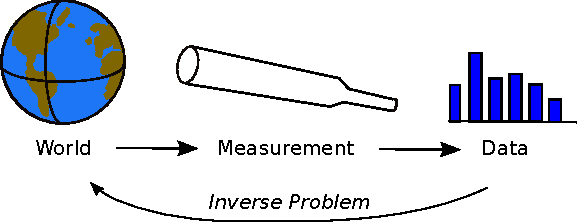
\includegraphics[width=0.9\linewidth]{inverseProblem}
\end{center}
\keywords{Least Squares, Under-constrained Systems, Ill-conditioning}
%%%%%%%%%%%%%%%%%%%%%%% Next Slide %%%%%%%%%%%%%%%%%%%%%%%
\renewcommand{\Outline}{%
\begin{slide}
\section[1]{Outline}

\begin{minipage}{12cm}
  \begin{enumerate}\squeeze
    \outlineitem{Least Squares}{leastsquares}
    \outlineitem{Under-constrained Systems}{underconstrained}
    \outlineitem{Ill-conditioning}{illconditioning}
  \end{enumerate}
\end{minipage}\hfill
\begin{minipage}{10cm}
  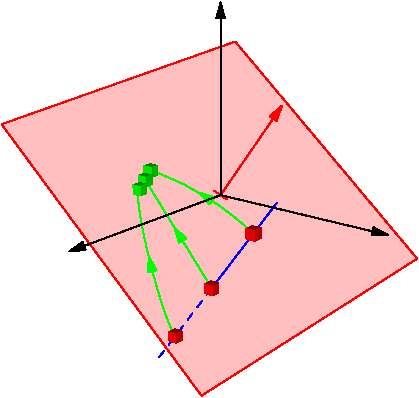
\includegraphics[height=10cm]{ill_conditioned_map}
\end{minipage}
\end{slide}
\addtocounter{outlineitem}{1}
}

\setcounter{outlineitem}{1}
\Outline
\toptarget{firstoutline}
%%%%%%%%%%%%%%%%%%%%%%% Next Slide %%%%%%%%%%%%%%%%%%%%%%%

\begin{slide}
\section[-2]{Transforming Data}

\begin{PauseHighLight}
  \begin{itemize}
  \item In the last lecture we spent time developing a sophisticated view
    of vector spaces and operators\pause
  \item At a mathematical level machine learning can be viewed as
    performing an inverse mapping
    \begin{center}
      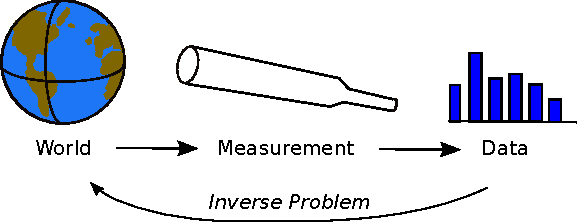
\includegraphics[width=12cm]{inverseProblem}\pause
    \end{center}
  \item Although our mappings are not necessarily linear in either
    direction we learn a lot by understanding linear operators\pause
  \end{itemize}
\end{PauseHighLight}



\end{slide}
%%%%%%%%%%%%%%%%%%%%%%% Next Slide %%%%%%%%%%%%%%%%%%%%%%%

\begin{slide}
\section{Inverse Problems}

\begin{PauseHighLight}
  \begin{itemize}
  \item Given $m$ observations $\{(\bm{x}_k, y_k)| k=1,\ldots,m\}$, find
    the $p$ unknowns $\bm{w}=(w_1,w_2, \ldots, w_p)^\tr$ such that
    $\bm{x}_k^\tr \bm{w} = y_k$\pause
\item Define the \textit{design matrix} as the matrix of feature vectors
  \begin{displaymath}
    \mat{X} = 
    \begin{pmatrix}
      \bm{x}_1^\tr \\ \bm{x}_2^\tr \\ \vdots \\ \bm{x}_m^\tr
    \end{pmatrix} =
    \begin{pmatrix}
      x_{11} & x_{12} & \cdots & x_{1p}\\
      x_{21} & x_{22} & \cdots & x_{2p}\\
      \vdots & \vdots & \ddots & \vdots \\
      x_{m1} & x_{m2} & \cdots & x_{mp}
    \end{pmatrix}\pause
  \end{displaymath}
\item and the target vector $\bm{y} = (y_1, y_2, \cdots, y_m)^\tr$\pause
\item Then $\bm{y} = \mat{X} \bm{w}$ and if $m=p$ (and $\mat{X}$ is
  invertible) $\bm{w} = \mat{X}^{-1} \bm{y}$\pause
\end{itemize}

\end{PauseHighLight}
\end{slide}

%%%%%%%%%%%%%%%%%%%%%%% Next Slide %%%%%%%%%%%%%%%%%%%%%%%

\begin{slide}
\section[-2]{Linear Regression}

\pb
\begin{itemize}\squeeze
\item $\bm{x}_k^\tr \bm{w}$ depends on distance from the plane orthogonal to $\bm{w}$\pauseh\pauselevel{=1}
\vspace*{-1cm}
\begin{center}
\multipdf[height=9.5cm]{linearRegression}\pause\\
\vspace*{-0.5cm}
\end{center}
\item If $m>p$ then $\mat{X}$ isn't square so doesn't have an inverse\pauseh
\item Worse, unless the data is exact, $\bm{y} \approx \mat{X}
  \bm{w}\Rightarrow$ no exact ``solution''\pauseh
\item Problem solved by Gauss to predict the orbit of the asteroid Ceres\pauseh
\end{itemize}
\end{slide}

%%%%%%%%%%%%%%%%%%%%%%% Next Slide %%%%%%%%%%%%%%%%%%%%%%%

\begin{slide}
\section[-1.5]{Linear Least Squares}

\begin{PauseHighLight}

\begin{itemize}\squeeze
\item The error of input pattern $\bm{x}_k$ is
  \begin{displaymath}
    \epsilon_k  = \bm{x}_k^\tr \bm{w}-y_k\pause
  \end{displaymath}
\item We can define the error vector
  \begin{displaymath}
    \bm{\epsilon} = \mat{X} \bm{w} - \bm{y}
  \end{displaymath}
(note that $\epsilon_k = \bm{x}_k^\tr \bm{w} -y_k$)\pause
\item The squared loss
  \begin{displaymath}
    L(\bm{w}|\mathcal{D}) =
    \sum_{k=1}^m\left(\bm{x}_k^\tr \bm{w}-y_k\right)^2
    = \sum_{k=1}^m \epsilon_k^2 = \| \bm{\epsilon} \|^2 \pause
  \end{displaymath}
\item Minimising this loss is known as the least squares problem\pause
\end{itemize}

\end{PauseHighLight}
\end{slide}

%%%%%%%%%%%%%%%%%%%%%%% Next Slide %%%%%%%%%%%%%%%%%%%%%%%

\begin{slide}
\section[-2]{Finding a Minimum}

\pb \pause
  \begin{itemize}
  \item At a minimum of a one-dimensional function, $f(x)$, we have
    $f'(x)=0$\pauseh
    \begin{center}
      \multipdf[width=0.5\linewidth]{gradient}\pause
    \end{center}
  \item At a minimum of an $n$-dimensional function $f(\bm{x})$
    we have the set of equations
    \begin{align*}
      \frac{\partial f(\bm{x})}{\partial x_i}=0 
      \quad \forall i=1,\ldots, n\pause
    \end{align*}
  \end{itemize}

\end{slide}


%%%%%%%%%%%%%%%%%%%%%%% Next Slide %%%%%%%%%%%%%%%%%%%%%%%

\begin{slide}
\section{Least Squares Solution}

\begin{PauseHighLight}

\begin{itemize}\squeeze
\item The least squares solution is given by
  \begin{align*}
    \grad L(\bm{w}|\mathcal{D}) &= \grad \|\bm{\epsilon}\|^2 \pause
                                  = \grad \| \mat{X} \bm{w} - \bm{y}\|^2 \pause \\
    &= \grad \left(\bm{w}^\tr
      \mat{X}^\tr\mat{X} \, \bm{w} -  2 \bm{w}^\tr\mat{X}^\tr \bm{y} +
      \bm{y}^\tr  \bm{y}\right)\pause\\
    &= 2 \left( \mat{X}^\tr\mat{X}\, \bm{w} - \mat{X}^\tr
      \bm{y}\right)\pause = 0 \pause
  \end{align*}
\item Or
  \begin{displaymath}
    \bm{w} = \left(\mat{X}^\tr\mat{X}\right)^{-1} \mat{X}^\tr \bm{y}\pause
    = \mat{X}^{+} \bm{y}
  \end{displaymath}
\item $\mat{X}^{+} = \left(\mat{X}^\tr\mat{X}\right)^{-1} \mat{X}^\tr$ is
  known as the pseudo-inverse\pause
\end{itemize}

\end{PauseHighLight}
\end{slide}

%%%%%%%%%%%%%%%%%%%%%%% Next Slide %%%%%%%%%%%%%%%%%%%%%%%

\begin{slide}
\section[-1]{Missing Bits of the Mathematics}

\begin{PauseHighLight}
  \begin{itemize}
  \item Note that $\len{\bm{a}}^2 = \bm{a}^\tr \bm{a} = \sum\limits_i a_i^2$\pause
    \begin{align*}
      \| \mat{X} \bm{w} - \bm{y}\|^2 &= (\mat{X} \bm{w} -
      \bm{y})^\tr(\mat{X} \bm{w} - \bm{y})\pause = (\bm{w}^\tr \mat{X}
                                       ^\tr - \bm{y}^\tr)(\mat{X}
                                       \bm{w} - \bm{y})\pauseb\\
      &=\bm{w}^\tr
      \mat{X}^\tr\mat{X} \, \bm{w} -  2 \bm{w}^\tr\mat{X}^\tr \bm{y} +
      \bm{y}^\tr  \bm{y}\pauseb\pauselevel{=4}
    \end{align*}
  \item Where we have used $\bm{w}^\tr\mat{X}^\tr \bm{y} =
    \bm{y}^\tr\mat{X} \bm{w}$\pause{}, $\sum\limits_{i,j} w_i X_{ji} y_j
    = \sum\limits_{i,j} y_i X_{ij} w_j$\pauseb
  \item Also $\grad \bm{w}^\tr \mat{M}\, \bm{w} = \mat{M}\,\bm{w} +
    \mat{M}^\tr\, \bm{w}\pause = (\mat{M} + \mat{M}^\tr)\, \bm{w}$\pauseb
  \item If $\mat{M}=\mat{M}^\tr$ (i.e.{} $\mat{M}$ is symmetric) then
    $\grad \bm{w}^\tr \mat{M}\, \bm{w} = 2\,\mat{M}\,\bm{w}$\pause
  \item As $(\mat{A}\mat{B})^\tr = \mat{B}^\tr \mat{A}^\tr$ then $(\mat{X}^\tr\mat{X})^\tr = \mat{X}^\tr\mat{X}^{\tr\tr}\pause=\mat{X}^\tr\mat{X}$ and
    $\mat{X}^\tr\mat{X}$ is symmetric\pauseb
  \end{itemize}
\end{PauseHighLight}

\end{slide}


%%%%%%%%%%%%%%%%%%%%%%% Next Slide %%%%%%%%%%%%%%%%%%%%%%%
\Outline % Under-constrained Systems
%%%%%%%%%%%%%%%%%%%%%%% Next Slide %%%%%%%%%%%%%%%%%%%%%%%

\begin{slide}
\section{Solving Inverse Problems}

\begin{PauseHighLight}
  \begin{itemize}
  \item Gauss showed us how to solve \emph{over-constrained} problems
    (we have more observations than parameters)\pause
  \item We seek a solution which isn't necessarily exact but minimises
    an error\pause
  \item But, what if we have more parameters than observations?\pause
  \item That is, we are \emph{under-constrained}\pause
  \item Note that in some directions you might be over-constrained and
    in other directions under-constrained\pause
  \item This is very typical of most machine learning problems\pauseb
  \end{itemize}
\end{PauseHighLight}

\end{slide}

%%%%%%%%%%%%%%%%%%%%%%% Next Slide %%%%%%%%%%%%%%%%%%%%%%%

\begin{slide}
\section[-2]{Under-constrained Systems}

\pb
  \begin{itemize}\squeeze
  \item If we have fewer data points than parameters then there will be
    multiple solutions, e.g.{} fitting
    $y = w_0 + w_1\,x + \cdots + w_5\,x^5$ to 4 points\pauseh
    \begin{center}
      \multipdf[height=10cm]{underConstrainedCurves}\pause
    \end{center}
  \item Every curve fits the data exactly, so which one should we
    choose?\pause
  \end{itemize}

\end{slide}


%%%%%%%%%%%%%%%%%%%%%%% Next Slide %%%%%%%%%%%%%%%%%%%%%%%

\begin{slide}
\section[-2]{What is the Inverse?}

\pb
  \begin{itemize}
  \item Many points can map to the same point\pause
    \begin{center}
      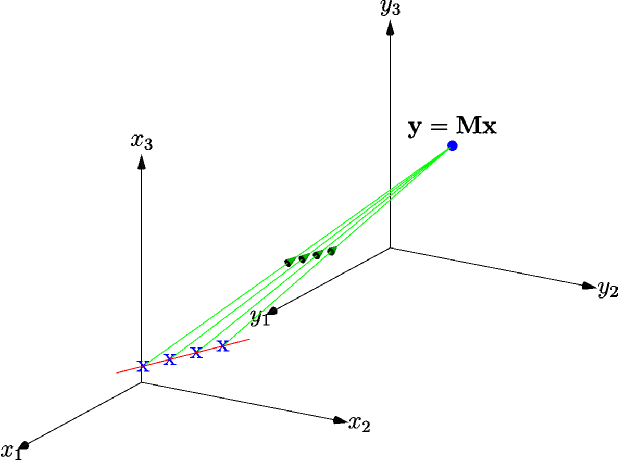
\includegraphics[width=0.75\linewidth]{underConstrained0}\mypl{1}
      \llap{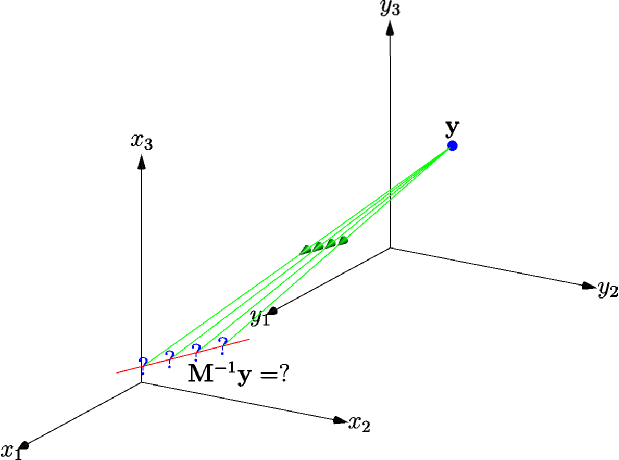
\includegraphics[width=0.75\linewidth]{underConstrained1}}\mypl{2}
    \end{center}
  \end{itemize}

\end{slide}

%%%%%%%%%%%%%%%%%%%%%%% Next Slide %%%%%%%%%%%%%%%%%%%%%%%

\begin{slide}
\section[-1]{Under-constrained Systems}

\begin{PauseHighLight}
  \begin{itemize}
  \item The system is \emph{under-constrained}\pause
  \item We have more unknowns than equations\pause
  \item The inverse is not unique\pause
  \item Solving the inverse problem ($\bm{w} =
    \left(\mat{X}^\tr\mat{X}\right)^{-1} \mat{X}^\tr \bm{y}$) is said 
    to be \emph{ill-posed}\pause
  \item The inverse $\left(\mat{X}^\tr\mat{X}\right)^{-1}$ doesn't
    exist\pause 
  \item If we have a complicated learning machine and not sufficient
    data we often end up with an ill-posed inverse problem (there are lots
    of sets of parameters that explain the data)\pause
  \end{itemize}
\end{PauseHighLight}

\end{slide}

%%%%%%%%%%%%%%%%%%%%%%% Next Slide %%%%%%%%%%%%%%%%%%%%%%%

\begin{slide}
\section{Handling Under-constrained Systems}

\begin{PauseHighLight}
  \begin{itemize}
  \item The issue with under-constrained systems is not that there is
    no solution\pause
  \item There is a whole family of solutions\pause, so which one
    should we pick\pauseb
  \item William of Ockham in the 14th century postulated that the
    ``simplest solution'' is likely to be the correct solution\pause
  \item How we determine the simplest solution is a bit of a black
    art\pause
  \item However, for linear regression, adding an $L_2$ regulariser
    makes the solution unique
    \begin{align*}
      L_{full} = L_{fit}(\bm{w}) + \eta \, \len{\bm{w}}^2_2\pause
    \end{align*}
  \end{itemize}
\end{PauseHighLight}

\end{slide}

%%%%%%%%%%%%%%%%%%%%%%% Next Slide %%%%%%%%%%%%%%%%%%%%%%%
\Outline % Ill-conditioning
%%%%%%%%%%%%%%%%%%%%%%% Next Slide %%%%%%%%%%%%%%%%%%%%%%%

\begin{slide}
  \section{Ill-Conditioning}

  \begin{PauseHighLight}
    \begin{itemize}
    \item Singular matrices are rare (although they occur when we don't
      have enough data), but matrices that are close to
      being singular are common\pause
    \item If a matrix is close to singular it is ill-conditioned\pause
    \item Ill-conditioned matrices have some eigenvalues that are tiny compared with the largest\pause
    \item All points get squashed towards a lower-dimensional subspace (a plane in 3-D)\pause
    \item Large matrices are very often ill-conditioned\pause
    \end{itemize}
  \end{PauseHighLight}
\end{slide}

%%%%%%%%%%%%%%%%%%%%%%% Next Slide %%%%%%%%%%%%%%%%%%%%%%%

\begin{slide}
  \section[-1]{Ill-Conditioned Matrices}

  \begin{PauseHighLight}

    \begin{center}
      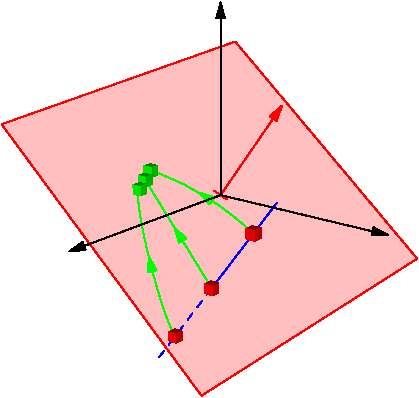
\includegraphics[height=15cm]{ill_conditioned_map}
    \end{center}

  \end{PauseHighLight}
\end{slide}

%%%%%%%%%%%%%%%%%%%%%%% Next Slide %%%%%%%%%%%%%%%%%%%%%%%

\begin{slide}
\section[-1]{A Worked Example}

\begin{PauseHighLight}
  \begin{itemize}\squeeze
  \item Two data points and two features that are almost the same
    \begin{displaymath}
      \mat{X} =
      \begin{pmatrix}
        1 & 1 \\ 1 & 1.001
      \end{pmatrix},
      \qquad
      \bm{y} = \begin{pmatrix} 2 \\ 2.001 \end{pmatrix}
      \quad\Rightarrow\quad
      \bm{w} = \begin{pmatrix} 1 \\ 1 \end{pmatrix}\pause
    \end{displaymath}
  \item Change $y_2$ by $0.001$ (i.e.{} $0.05\%$)
    \begin{displaymath}
      \bm{y} = \begin{pmatrix} 2 \\ 2.002 \end{pmatrix}
      \quad\Rightarrow\quad
      \bm{w} = \begin{pmatrix} 0 \\ 2 \end{pmatrix}\pause
    \end{displaymath}
  \item The prediction for a new input $\bm{x}=(1,0)^\tr$ jumps from 1 to 0\pause
  \item The eigenvalues of $\mat{X}$ are about $2$ and $0.0005$\pause
  \item $\bm{w}$ moved along $(-1,1)^\tr$, the direction with the tiny
    eigenvalue, which the data hardly constrains\pause
  \end{itemize}
\end{PauseHighLight}
\end{slide}

%%%%%%%%%%%%%%%%%%%%%%% Next Slide %%%%%%%%%%%%%%%%%%%%%%%

\begin{slide}
\section{Ill-Conditioning in ML}

\begin{PauseHighLight}
  \begin{itemize}
  \item Ill-conditioning in machine learning occurs when a very small
    change in the learning data causes a large change in the predictions
    of the learning machine\pause
  \item In linear regression the matrix $\mat{X}^\tr\mat{X}$ is typically
    ill-conditioned when we have roughly as many data points as parameters\pause
  \item Much of machine learning is concerned with making learning
    machines better conditioned\pause
  \item Adding regularisers is one approach to achieve this\pause
  \end{itemize}
\end{PauseHighLight}

\end{slide}

%%%%%%%%%%%%%%%%%%%%%%% Next Slide %%%%%%%%%%%%%%%%%%%%%%%

\begin{slide}
\section[-1]{Where Does Ill-Conditioning Come From?}

\begin{PauseHighLight}
  \begin{itemize}
  \item Too little data: about as many data points as parameters\pause
  \item Nearly collinear features, e.g.{} floor area and number of
    rooms, or height measured in both cm and inches\pause
    \begin{itemize}
    \item The columns of $\mat{X}$ are nearly parallel so the data
      cannot tell us how to share the weight between them\pause
    \end{itemize}
  \item Polynomial features $x, x^2, \ldots, x^9$ for $x\in[0,1]$ all
    look alike: the eigenvalues of $\mat{X}^\tr\mat{X}$ span about
    13 orders of magnitude\pause
  \item Features on very different scales (income in pounds and age in
    years)---easily fixed by standardising the features\pause
  \end{itemize}
\end{PauseHighLight}

\end{slide}

%%%%%%%%%%%%%%%%%%%%%%% Next Slide %%%%%%%%%%%%%%%%%%%%%%%

\begin{slide}
\section[-1]{Least Squares in Practice}

\begin{PauseHighLight}
  \begin{itemize}
  \item $\bm{w} = \left(\mat{X}^\tr\mat{X}\right)^{-1} \mat{X}^\tr
    \bm{y}$ is for understanding, not for computing\pause
  \item Never compute $\left(\mat{X}^\tr\mat{X}\right)^{-1}$; use a
    least squares solver such as \texttt{np.linalg.lstsq(X, y)}, which
    works with $\mat{X}$ directly\pause
  \item Forming $\mat{X}^\tr\mat{X}$ squares the ratio of largest to
    smallest eigenvalues: $10^8$ becomes $10^{16}$, beyond the
    $\sim$16 significant figures of a double\pause
  \item Standardise features (zero mean, unit variance) before
    fitting\pause
  \item When $m<p$, \texttt{lstsq} returns the solution with the
    smallest $\len{\bm{w}}$---one version of the ``simplest''
    solution (we will see why when we meet the SVD)\pause
  \end{itemize}
\end{PauseHighLight}

\end{slide}

%%%%%%%%%%%%%%%%%%%%%%% Next Slide %%%%%%%%%%%%%%%%%%%%%%%

\begin{slide}
\section[-1]{Three Regimes}

\begin{PauseHighLight}

  \begin{center}
    \renewcommand{\arraystretch}{1.2}
    \begin{tabular}{|l|p{6.0cm}|p{4.9cm}|p{6.7cm}|}\hline
      & $m>p$ \newline \mbox{over-constrained} & $m=p$ & $m<p$ \newline
      \mbox{under-constrained} \\ \hline
      Exact fit? & usually not & yes & yes, many \\ \hline
      Unique? & yes (usually) & yes (usually) & no \\ \hline
      Method & least squares & $\bm{w}=\mat{X}^{-1}\bm{y}$ & pick ``simplest'' \\ \hline
    \end{tabular}\pause
  \end{center}
  \begin{itemize}
  \item Real problems mix these: over-constrained in some directions
    and (nearly) under-constrained in others\pause
  \item The nearly under-constrained directions make the problem
    ill-conditioned\pause
  \end{itemize}
\end{PauseHighLight}

\end{slide}

%%%%%%%%%%%%%%%%%%%%%%% Next Slide %%%%%%%%%%%%%%%%%%%%%%%

\begin{slide}
\section{Summary}

\begin{PauseHighLight}
  \begin{itemize}
  \item Linear mappings are commonly used in machine learning algorithms
    such as regression\pause
  \item Systems can be over-constrained, under-constrained or
    ill-conditioned---often all at once\pause
  \item We will often meet the pseudo-inverse involving inverting
    $\mat{X}^\tr\,\mat{X}$\pause 
  \item Inverting an ill-conditioned $\mat{X}^\tr\,\mat{X}$ amplifies noise in the data\pause
  \end{itemize}
\end{PauseHighLight}

\end{slide}


%%% Local Variables:
%%% TeX-master: "lectures"
%%% End:

\end{document}
